\mychapter{3}{Input variable analysis}
\label{sec:unchapitre}

A large set of variables is available from CMS data. MVA training can be time consumming and the "dimensionality curse" forces us to select only a few of them based on two main criteria :
\begin{description}
    \item [Background vs Signal discrimination :] Variables with most differences of shape for background and signal will be picked.
    \item [Low correlation between variables :] Needed in order to reduce redundancy of input data and thus will permit
    to reduce MVA complexity (for example number of hidden neurons in ANN).
\end{description}

reference \cite{CMS2015}.

\section{Background vs Signal discrimination}

It is necessary to pick the smallest set of input variable for the MVA. This selection is done by looking at variable shape for background and signal data from MC simulation.

\begin{figure}[ht]
  \centering
  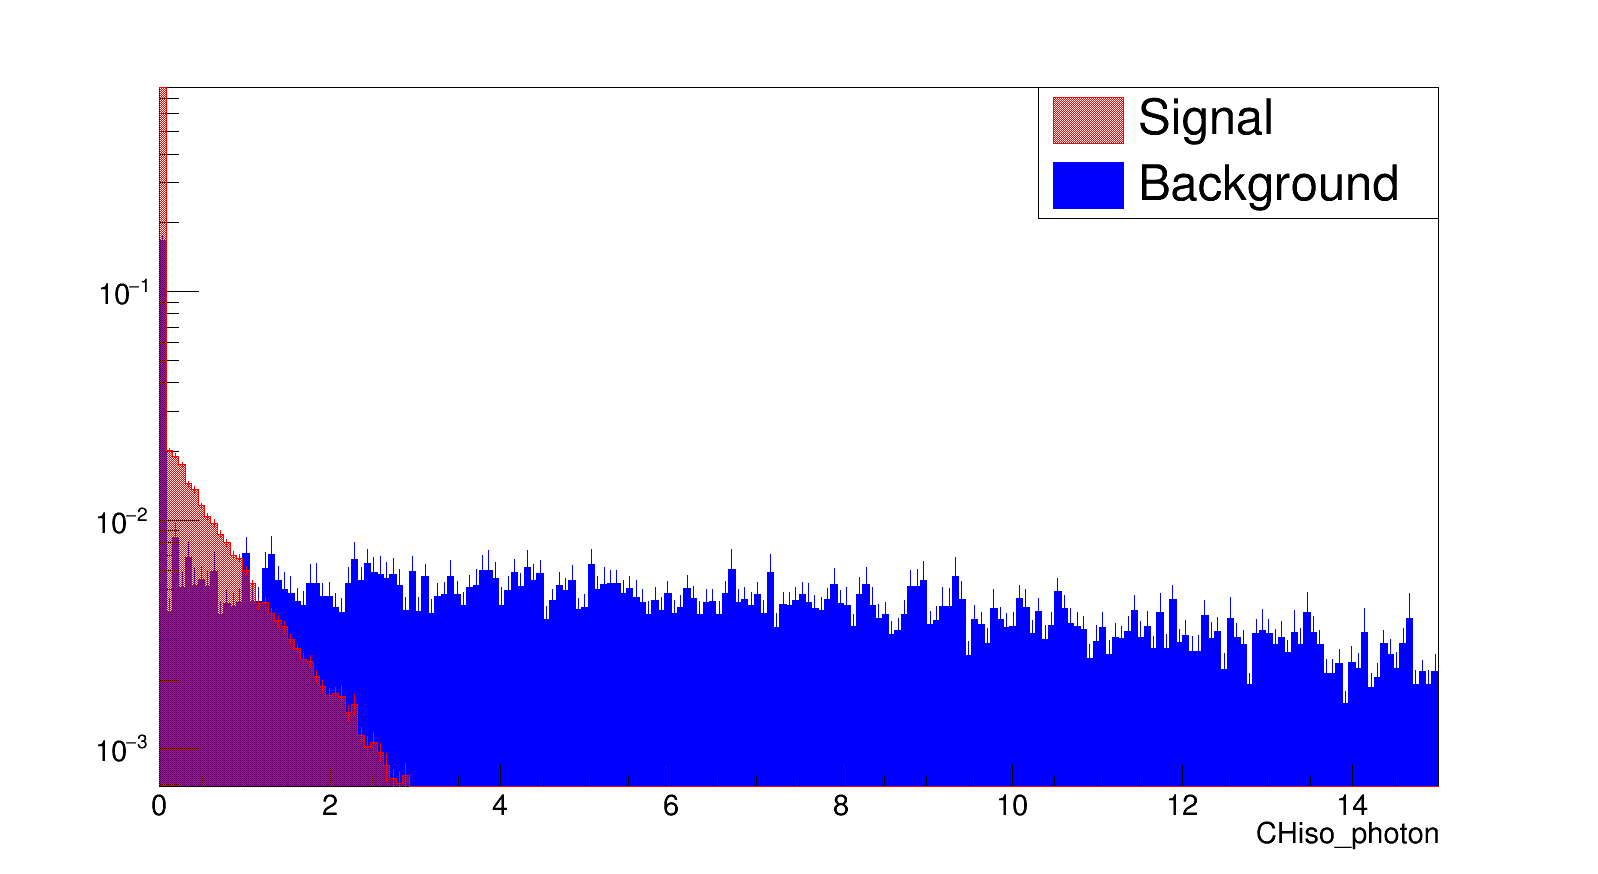
\includegraphics[width=0.8\textwidth]{CHiso_photon}\\[1cm]
  \caption{Charge hadron isolation for background and signal, here is a good discrimination between them}
  \label{fig:une-image}
\end{figure}


\section{Variable correlations}

Training data needed-quantity increases with network complexity. So correlation between variables must be avoided in order to get the minimum redundancy.

%%% Local Variables: 
%%% mode: latex
%%% TeX-master: "isae-report-template"
%%% End: 
